\chapter{Resultados}
\label{cap:resultados}

\section{Cohortes evaluables y curación LLM}
\label{sec:res_cohortes}

De las 11 cohortes GEO descargadas, 8 cumplen los criterios de inclusión
para la tarea tumor \emph{vs.} sano. Sobre estas 8 cohortes evaluables se
analizan 662 muestras (sanas + enfermas). Las 3 cohortes excluidas
(GSE30219, GSE50081 y GSE140797) no tienen controles sanos evaluables y no
permiten entrenar el clasificador; sus muestras tumorales sí se aprovechan
para engrosar el conjunto de entrenamiento en LODO. En total el pipeline
maneja 1157 muestras curadas por el LLM (219 sanas + 938 enfermas) sobre
1346 descargadas.

La tasa de éxito global de la curación LLM es del 85,9\,\%, con
9 cohortes por encima del 95\,\% y una única cohorte (GSE40791) por debajo
del 20\,\% debido a que los metadatos de esa serie son excepcionalmente
crípticos y el modelo declara la mayoría de muestras como
\emph{ambiguo}. La figura~\ref{fig:curacion} resume la tasa de éxito por
cohorte.

\begin{figure}[H]
  \centering
  
\includegraphics[width=0.85\linewidth]{figuras/fig_curacion_llm.pdf}
  \caption{Tasa de éxito de la curación LLM por cohorte. Barras verdes
  indican cohortes con curación superior al 40\,\% (umbral de inclusión).}
  \label{fig:curacion}
\end{figure}

\section{Clasificación tumor \emph{vs.} sano}
\label{sec:res_tvs}

Sobre las 8 cohortes evaluables, el clasificador de regresión logística L1
alcanza en validación externa LODO una AUC media de \textbf{0,925} y una
balanced accuracy media de \textbf{0,772}. Los valores por cohorte se
recogen en la tabla~\ref{tab:lodo_tvs}. La sensibilidad media es de 0,983
y la especificidad de 0,561, reflejando un modelo con capacidad
discriminativa alta pero un umbral de decisión que necesita recalibrarse
entre cohortes para equilibrar los dos tipos de error.

\begin{table}[H]
  \centering
  \small
  \caption{Rendimiento LODO para la tarea tumor \emph{vs.} sano.}
  \label{tab:lodo_tvs}
  \begin{tabular}{lrrrrrrr}
    \toprule
    \textbf{Cohorte test} & $n$ & \textbf{Sano} & \textbf{Enf.} & \textbf{AUC} & \textbf{Bal.\,acc.} & \textbf{Sens.} & \textbf{Espec.} \\
    \midrule
    GSE118370 & 12  & 6  & 6   & 1,000 & 0,917 & 1,000 & 0,833 \\
    GSE18842  & 91  & 45 & 46  & 1,000 & 0,889 & 1,000 & 0,778 \\
    GSE19188  & 156 & 65 & 91  & 0,984 & 0,904 & 0,978 & 0,831 \\
    GSE19804  & 120 & 60 & 60  & 0,984 & 0,775 & 1,000 & 0,550 \\
    GSE23066  & 10  & 5  & 5   & 0,440 & 0,500 & 1,000 & 0,000 \\
    GSE31210  & 246 & 20 & 226 & 0,993 & 0,943 & 0,993 & 0,885 \\
    GSE40791  & 12  & 10 & 2   & 0,500 & 0,500 & 1,000 & 0,000 \\
    GSE7670   & 15  & 8  & 7   & 1,000 & 0,750 & 1,000 & 0,500 \\
    \midrule
    \textbf{Media} & & & & \textbf{0,925} & \textbf{0,772} & \textbf{0,983} & \textbf{0,561} \\
    \bottomrule
  \end{tabular}
\end{table}

Todos los baselines mayoritarios informados quedan por debajo del
rendimiento del clasificador (media 0,609, ganancia media $+$0,163 en
balanced accuracy). Sólo dos cohortes (GSE23066 y GSE40791) presentan un
AUC por debajo de 0,7, ambas con un tamaño muestral escaso ($n \leq 12$).
La figura~\ref{fig:lodo_baseline} muestra visualmente la comparación entre
el modelo y el baseline por cohorte.

\begin{figure}[H]
  \centering
  
\includegraphics[width=0.85\linewidth]{figuras/fig_lodo_vs_baseline.pdf}
  \caption{Balanced accuracy del modelo en LODO frente al baseline
  mayoritario informado por cohorte.}
  \label{fig:lodo_baseline}
\end{figure}

La discrepancia entre AUC (0,925) y balanced accuracy (0,772) merece
comentario. El AUC mide la capacidad de \emph{ordenar} las muestras (dado
un par sano/enfermo aleatorio, la probabilidad de que el modelo asigne
mayor score al enfermo). La balanced accuracy depende además de la
elección del umbral de decisión. La figura~\ref{fig:auc_vs_balacc}
representa ambas métricas por cohorte y muestra un patrón consistente: la
firma ordena bien pero el umbral óptimo varía entre cohortes. Este
comportamiento es propio del desbalance del entrenamiento (938 tumores
frente a 219 controles curados en total) y es corregible mediante
recalibración isotónica o \emph{Platt scaling} por cohorte, sin necesidad
de reentrenar la firma.

\begin{figure}[H]
  \centering
  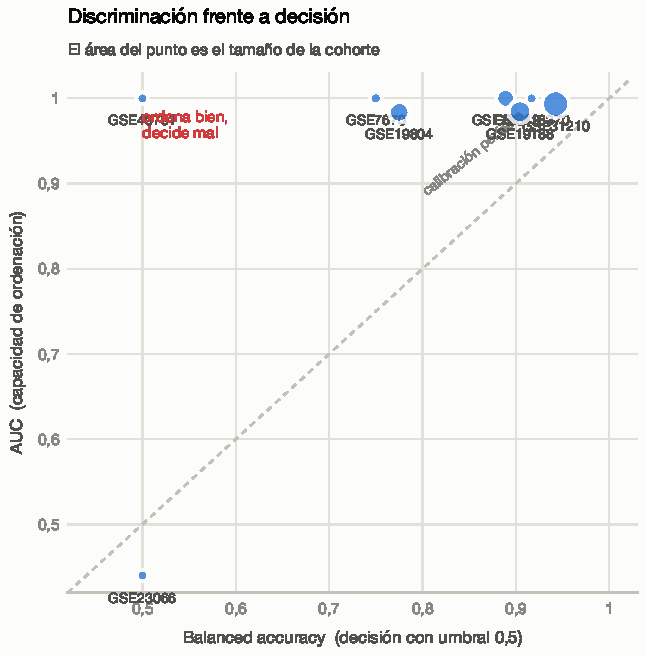
\includegraphics[width=0.85\linewidth]{figuras/fig_auc_vs_balacc.pdf}
  \caption{AUC frente a balanced accuracy por cohorte en LODO. La brecha
  vertical entre ambas cifras es proporcional a la necesidad de
  recalibración del umbral.}
  \label{fig:auc_vs_balacc}
\end{figure}

\section{Clasificación de subtipo histológico ADC \emph{vs.} SQC}
\label{sec:res_subtipo}

Sobre 3 cohortes independientes GPL570 (388 muestras totales validadas con
LODO), el clasificador alcanza AUC media \textbf{0,968} y balanced
accuracy \textbf{0,940}. La tabla~\ref{tab:lodo_sub} resume las cifras por
cohorte.

\begin{table}[H]
  \centering
  \small
  \caption{Rendimiento LODO para la tarea de subtipo ADC \emph{vs.} SQC.}
  \label{tab:lodo_sub}
  \begin{tabular}{lrrrrrrr}
    \toprule
    \textbf{Cohorte test} & $n$ & \textbf{ADC} & \textbf{SQC} & \textbf{AUC} & \textbf{Bal.\,acc.} & \textbf{Sens.\,SQC} & \textbf{Espec.\,ADC} \\
    \midrule
    GSE30219 & 146 & 85  & 61 & 0,996 & 0,967 & 0,934 & 1,000 \\
    GSE50081 & 170 & 127 & 43 & 0,911 & 0,887 & 0,837 & 0,937 \\
    GSE19188 & 72  & 45  & 27 & 0,998 & 0,967 & 1,000 & 0,933 \\
    \midrule
    \textbf{Media} & & & & \textbf{0,968} & \textbf{0,940} & \textbf{0,924} & \textbf{0,957} \\
    \bottomrule
  \end{tabular}
\end{table}

La tarea de subtipo se resuelve mucho mejor que la de tumor \emph{vs.}
sano, lo que era esperable: las diferencias transcripcionales entre ADC y
SQC son más profundas y menos condicionadas por el nivel de infiltración
tumoral en el tejido de la muestra.

\section{Firma génica validada}
\label{sec:res_firma}

Aplicando el criterio de consenso multi-cohorte descrito en el
capítulo~\ref{cap:metodos}, se obtiene una firma génica de
\textbf{1174 genes} replicados en las tres cohortes independientes, sobre
un total de 22\,880 genes evaluados. Esto representa una tasa de
replicación del 5,1\,\% del transcriptoma, cifra coherente con la
literatura de meta-análisis multi-cohorte en cáncer.

El top 10 de la firma, ordenado por $d$ media entre cohortes, es:
\gene{DSG3}, \gene{KRT5}, \gene{CALML3}, \gene{KRT6B}, \gene{PKP1},
\gene{FAT2}, \gene{DAPL1}, \gene{TRIM29}, \gene{CLCA2}, \gene{DSC3}. Los
diez genes corresponden a linaje celular epitelial escamoso puro: hay
tres desmosomas (\gene{DSG3}, \gene{DSC3}, \gene{PKP1}), cuatro queratinas
o proteínas relacionadas (\gene{KRT5}, \gene{KRT6B}, \gene{CALML3},
\gene{TRIM29}), y tres factores adicionales de diferenciación escamosa
(\gene{FAT2}, \gene{DAPL1}, \gene{CLCA2}).

\section{Panel mínimo}
\label{sec:res_panel}

El análisis de sensibilidad sobre distintos tamaños de panel produce la
curva de la figura~\ref{fig:panel_minimo}. El panel mínimo que se mantiene
a menos de 0,01 del AUC máximo alcanza \textbf{20 genes} con AUC
\textbf{0,966}, frente a los 1174 genes de la firma completa con AUC
\textbf{0,970}. Los 20 genes del panel mínimo son: \gene{DSG3},
\gene{KRT5}, \gene{CALML3}, \gene{KRT6B}, \gene{PKP1}, \gene{FAT2},
\gene{DAPL1}, \gene{TRIM29}, \gene{CLCA2}, \gene{DSC3}, \gene{S1PR5},
\gene{KRT6A}, \gene{KRT13}, \gene{SERPINB5}, \gene{TP63}, \gene{GJB5},
\gene{KRT16}, \gene{BNC1}, \gene{CERS3}, \gene{TMEM40}.

\begin{figure}[H]
  \centering
  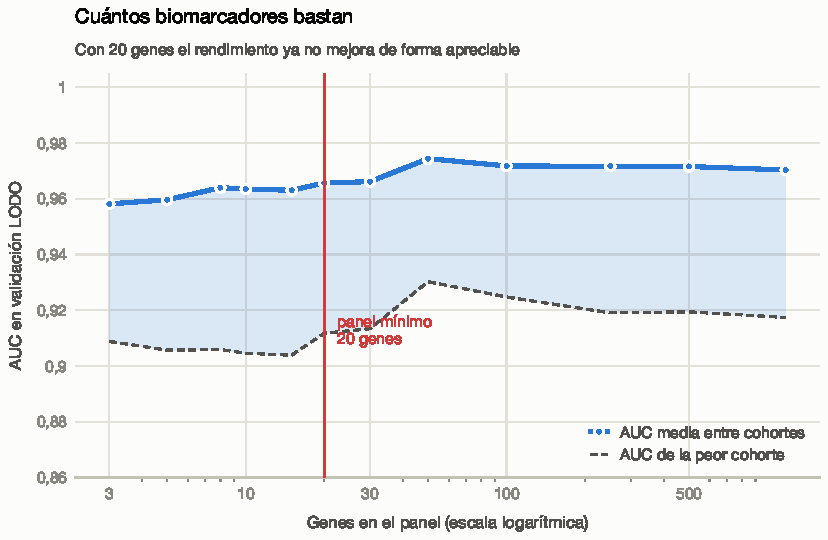
\includegraphics[width=0.85\linewidth]{figuras/fig_panel_minimo.pdf}
  \caption{AUC media LODO en función del tamaño del panel (genes ordenados
  por $d$ media de la firma validada). El panel mínimo (20 genes) captura
  el 99,6\,\% del AUC de la firma completa.}
  \label{fig:panel_minimo}
\end{figure}

Este panel de 20 genes es susceptible de ser medido mediante PCR
cuantitativa multiplex o por \emph{NanoString nCounter}, tecnologías con
tiempos de respuesta y coste unitario compatibles con la aplicación
clínica.

\section{Validación externa contra IHC clínica}
\label{sec:res_ihc}

De los 20 marcadores diagnósticos IHC del panel OMS, el framework
recupera \textbf{18} sin haberlos declarado durante el entrenamiento:

\begin{itemize}
  \item \textbf{Escamoso: 12 de 12 recuperados.} \gene{KRT5}, \gene{KRT6A},
  \gene{KRT6B}, \gene{KRT13}, \gene{KRT14}, \gene{TP63}, \gene{DSG3},
  \gene{DSC3}, \gene{SOX2}, \gene{PKP1}, \gene{CALML3}, \gene{S100A2}.
  Cobertura completa del panel escamoso.
  \item \textbf{Adenocarcinoma: 6 de 8 recuperados.} \gene{NAPSA},
  \gene{NKX2-1}, \gene{SFTPB}, \gene{SLC34A2}, \gene{MUC1},
  \gene{CEACAM6}. Los dos no recuperados son \gene{SFTPA1} y \gene{SFTPC},
  ambas proteínas del surfactante cuya expresión cae de forma más
  homogénea entre tumor y sano que otros marcadores alveolares, lo que las
  hace menos discriminantes en la comparación ADC \emph{vs.} SQC (donde
  ambos linajes están alterados respecto al alvéolo normal).
\end{itemize}

La recuperación completa del panel escamoso y de tres cuartas partes del
adenocarcinoma constituye una validación externa fuerte frente a un
estándar clínico independiente. Es especialmente significativo que el
framework no haya recibido información previa sobre estos marcadores: la
selección se realiza únicamente por criterio estadístico de consenso
multi-cohorte.

\section{Composición tisular dentro de los tumores}
\label{sec:res_composicion}

Un riesgo conocido en firmas de tumor \emph{vs.} sano es que el
clasificador acabe midiendo composición tisular más que biología tumoral
(un tumor con más estroma o más pulmón sano residual tiene un perfil
distinto del tumor puro). Para descartar este confundente se calcula la
correlación entre el score del clasificador y el contenido residual de
pulmón sano dentro de cada tumor, estimado mediante marcadores canónicos
de alvéolo (\gene{AGER}, \gene{CLDN18}, \gene{SFTPC}, \gene{FABP4},
\gene{WIF1}).

La correlación media es $\rho = -0{,}626$ sobre 4 cohortes con muestra
suficiente ($n \geq 20$ tumores). En la cohorte GSE31210 (n=226
tumores), la más grande, alcanza $\rho = -0{,}858$ con $p = 1{,}1 \times
10^{-66}$. La figura~\ref{fig:composicion} representa la relación por
cohorte.

\begin{figure}[H]
  \centering
  
\includegraphics[width=0.85\linewidth]{figuras/fig_composicion_tumores.pdf}
  \caption{Correlación entre el score del clasificador y el contenido
  residual de pulmón sano dentro de los tumores, por cohorte.}
  \label{fig:composicion}
\end{figure}

La correlación negativa indica que los tumores con \emph{menos} pulmón
sano residual obtienen scores más altos, lo que constituye un eje
biológico legítimo (pérdida gradual de arquitectura alvéolo-capilar
normal) y no un artefacto de composición.

\section{Interpretación biológica: dos ejes reales}
\label{sec:res_biologia}

La firma completa integra dos ejes biológicos identificables:

\begin{description}
  \item[Eje 1 — Pérdida de arquitectura alvéolo-capilar normal.] Los
  tumores con menor expresión de marcadores canónicos de alvéolo sano
  obtienen scores más altos del clasificador. Marcadores usados para
  definir el eje (no seleccionados por la firma): \gene{AGER},
  \gene{CLDN18}, \gene{SFTPC}, \gene{FABP4}, \gene{WIF1}.
  \item[Eje 2 — Actividad proliferativa aumentada.] Los tumores más
  proliferativos concentran valores más altos del score. Panel canónico de
  proliferación: \gene{MKI67}, \gene{TOP2A}, \gene{CCNB1}, \gene{BIRC5},
  \gene{AURKA}.
\end{description}

Ambos ejes son señal biológica reproducible, no artefacto. Aportan
mecanismo: la firma captura la transición del pulmón sano hacia un tejido
menos diferenciado y más proliferativo, que es precisamente la histología
del NSCLC.

\section{Histologías fuera del alcance de entrenamiento}
\label{sec:res_histologias}

El clasificador de subtipo se entrena únicamente con adenocarcinoma y
carcinoma escamoso. La figura~\ref{fig:histologias} muestra qué otras
histologías aparecen en las cohortes GEO y quedan explícitamente fuera del
entrenamiento.

\begin{figure}[H]
  \centering
  
\includegraphics[width=0.85\linewidth]{figuras/fig_histologias_excluidas.pdf}
  \caption{Histologías presentes en las cohortes GEO originales que
  quedaron fuera del entrenamiento del clasificador de subtipo.}
  \label{fig:histologias}
\end{figure}

Estas incluyen tumores neuroendocrinos (carcinoide típico y atípico,
microcítico, LCNE) y algunos carcinomas de células grandes. El framework
declara explícitamente este alcance: no se debe usar para triage
diagnóstico sobre casos sin diagnosticar hasta ampliar el entrenamiento
con esas clases.

\section{Análisis exploratorio por cohorte}
\label{sec:res_por_cohorte}

Con fines ilustrativos, se muestran los resultados del análisis
exploratorio para la cohorte GSE31210 (la mayor con controles sanos, 226
muestras enfermas y 20 sanas), que ejemplifica el tipo de figuras que el
pipeline genera para cada cohorte individualmente.

\begin{figure}[H]
  \centering
  \begin{subfigure}[t]{0.31\textwidth}
    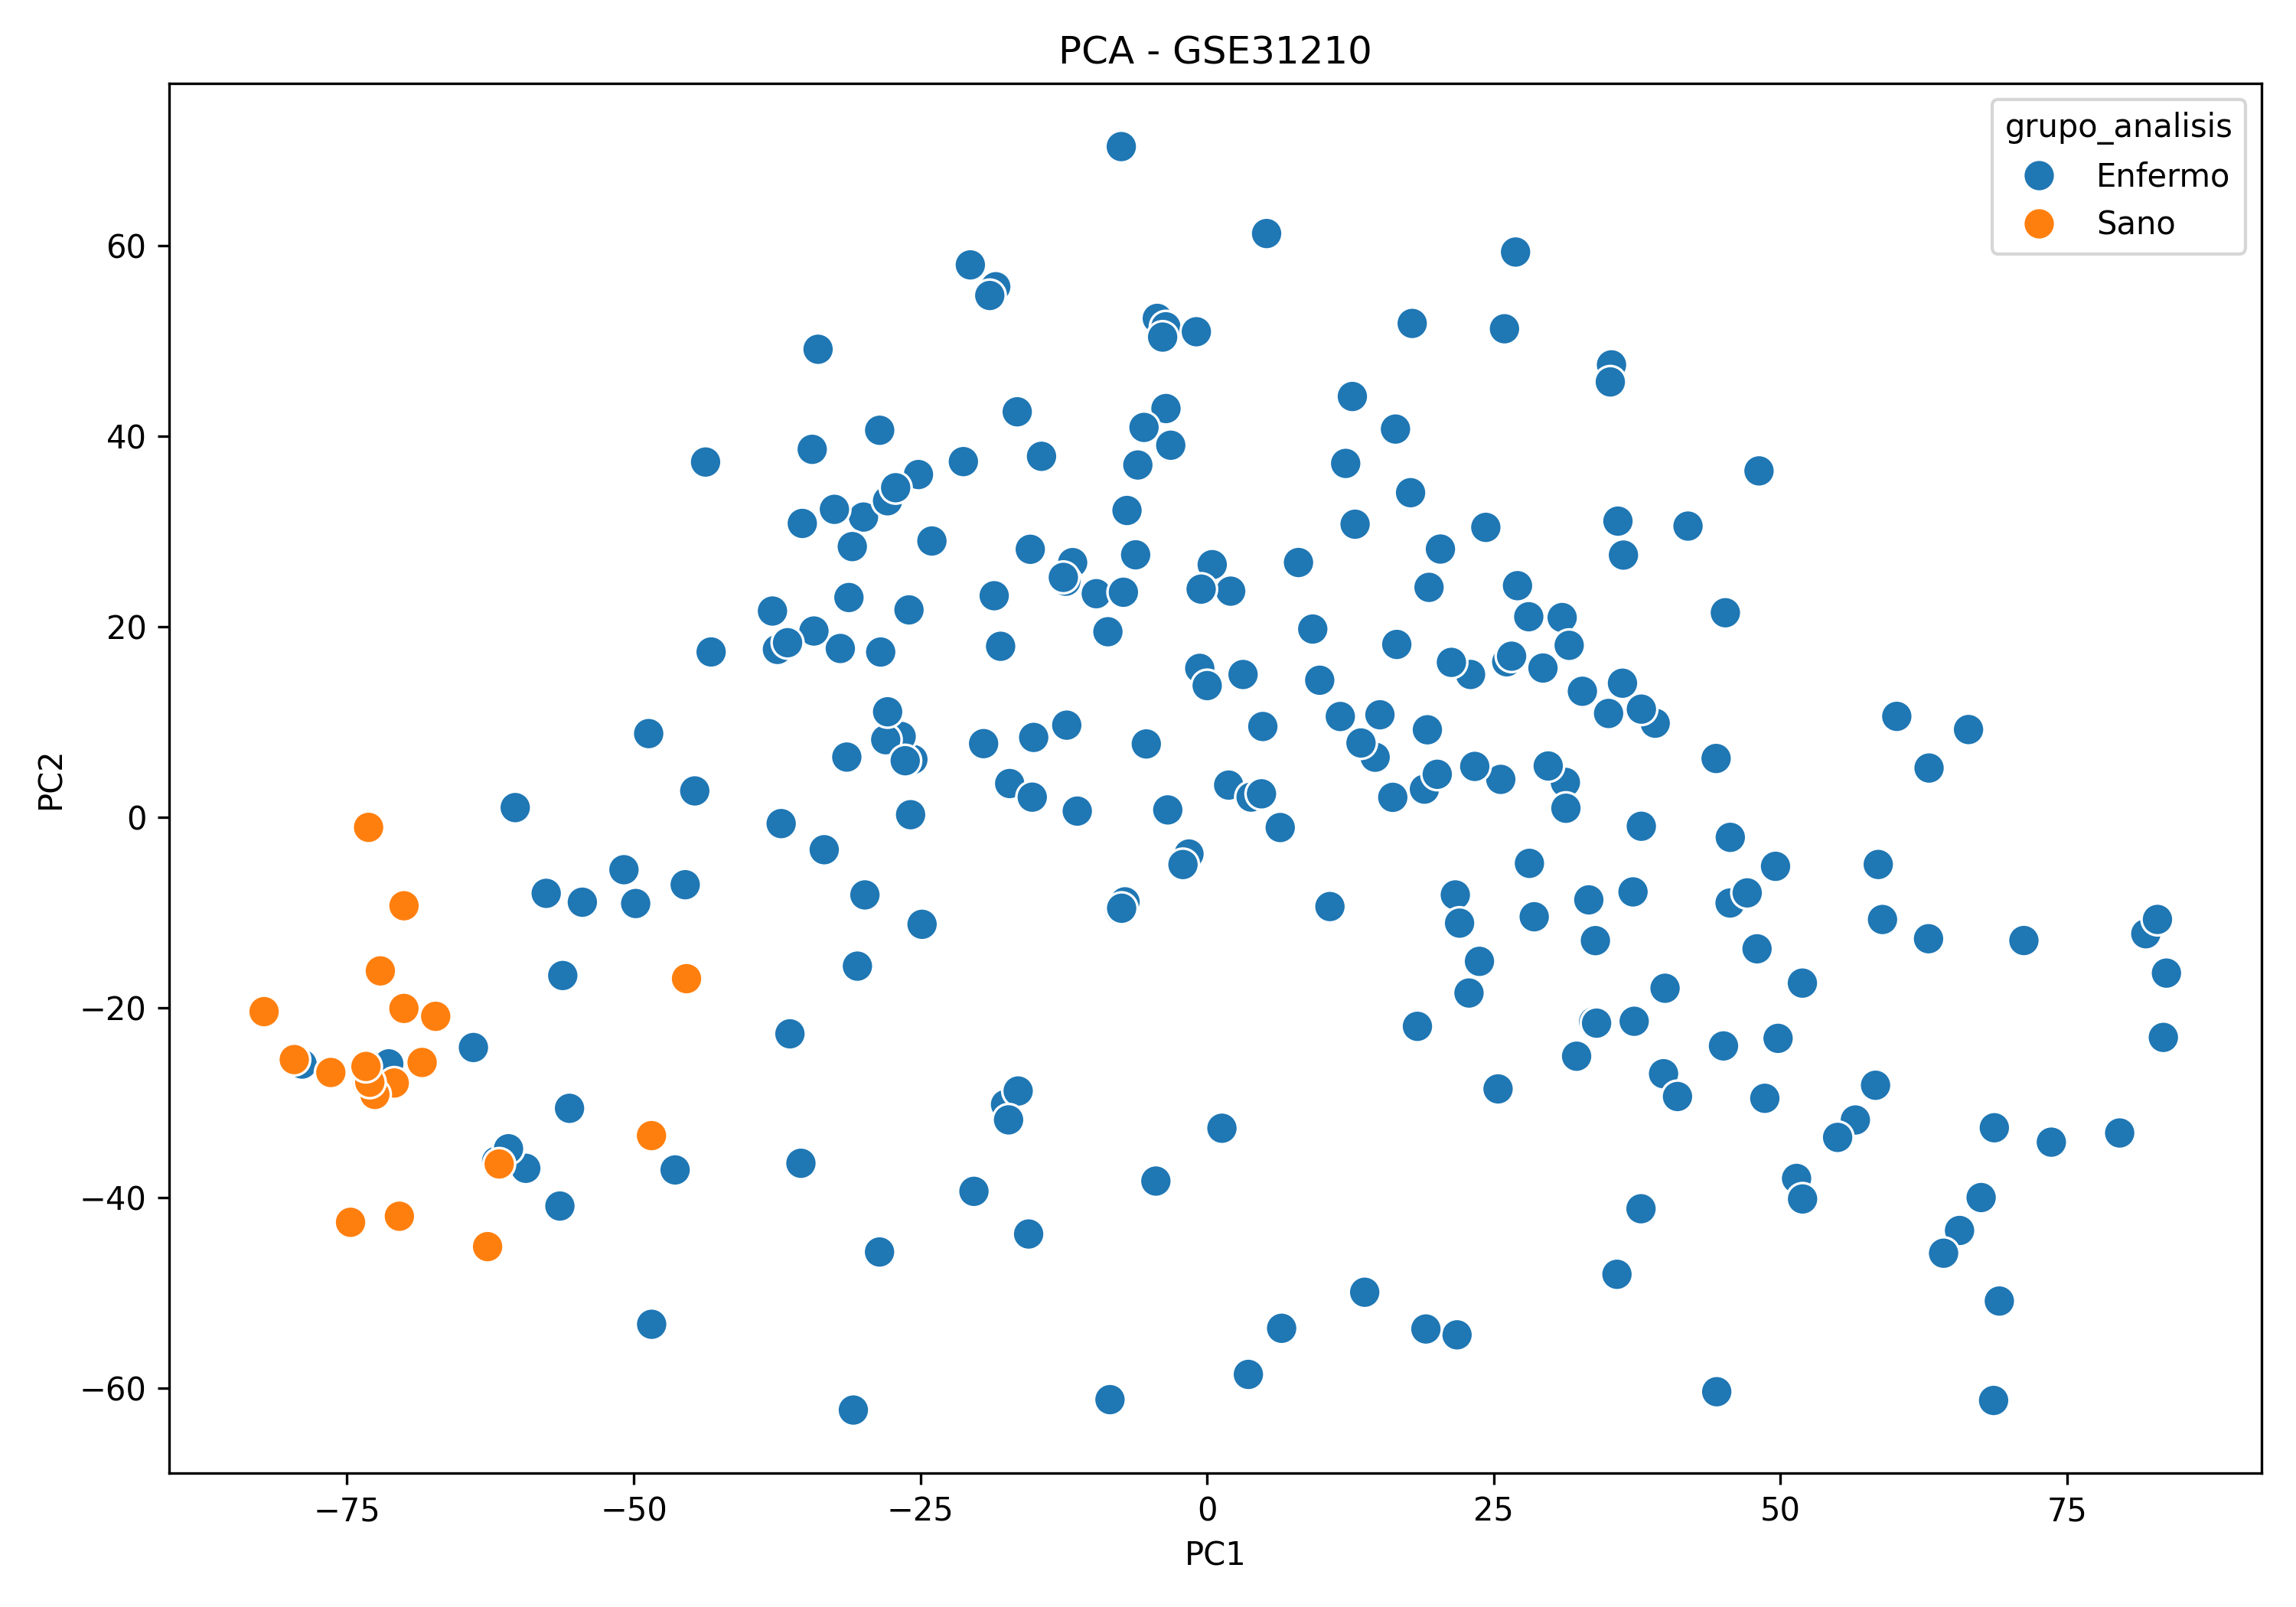
\includegraphics[width=\linewidth]{figuras/pca_gse31210.png}
    \caption{PCA}
  \end{subfigure}\hfill
  \begin{subfigure}[t]{0.31\textwidth}
    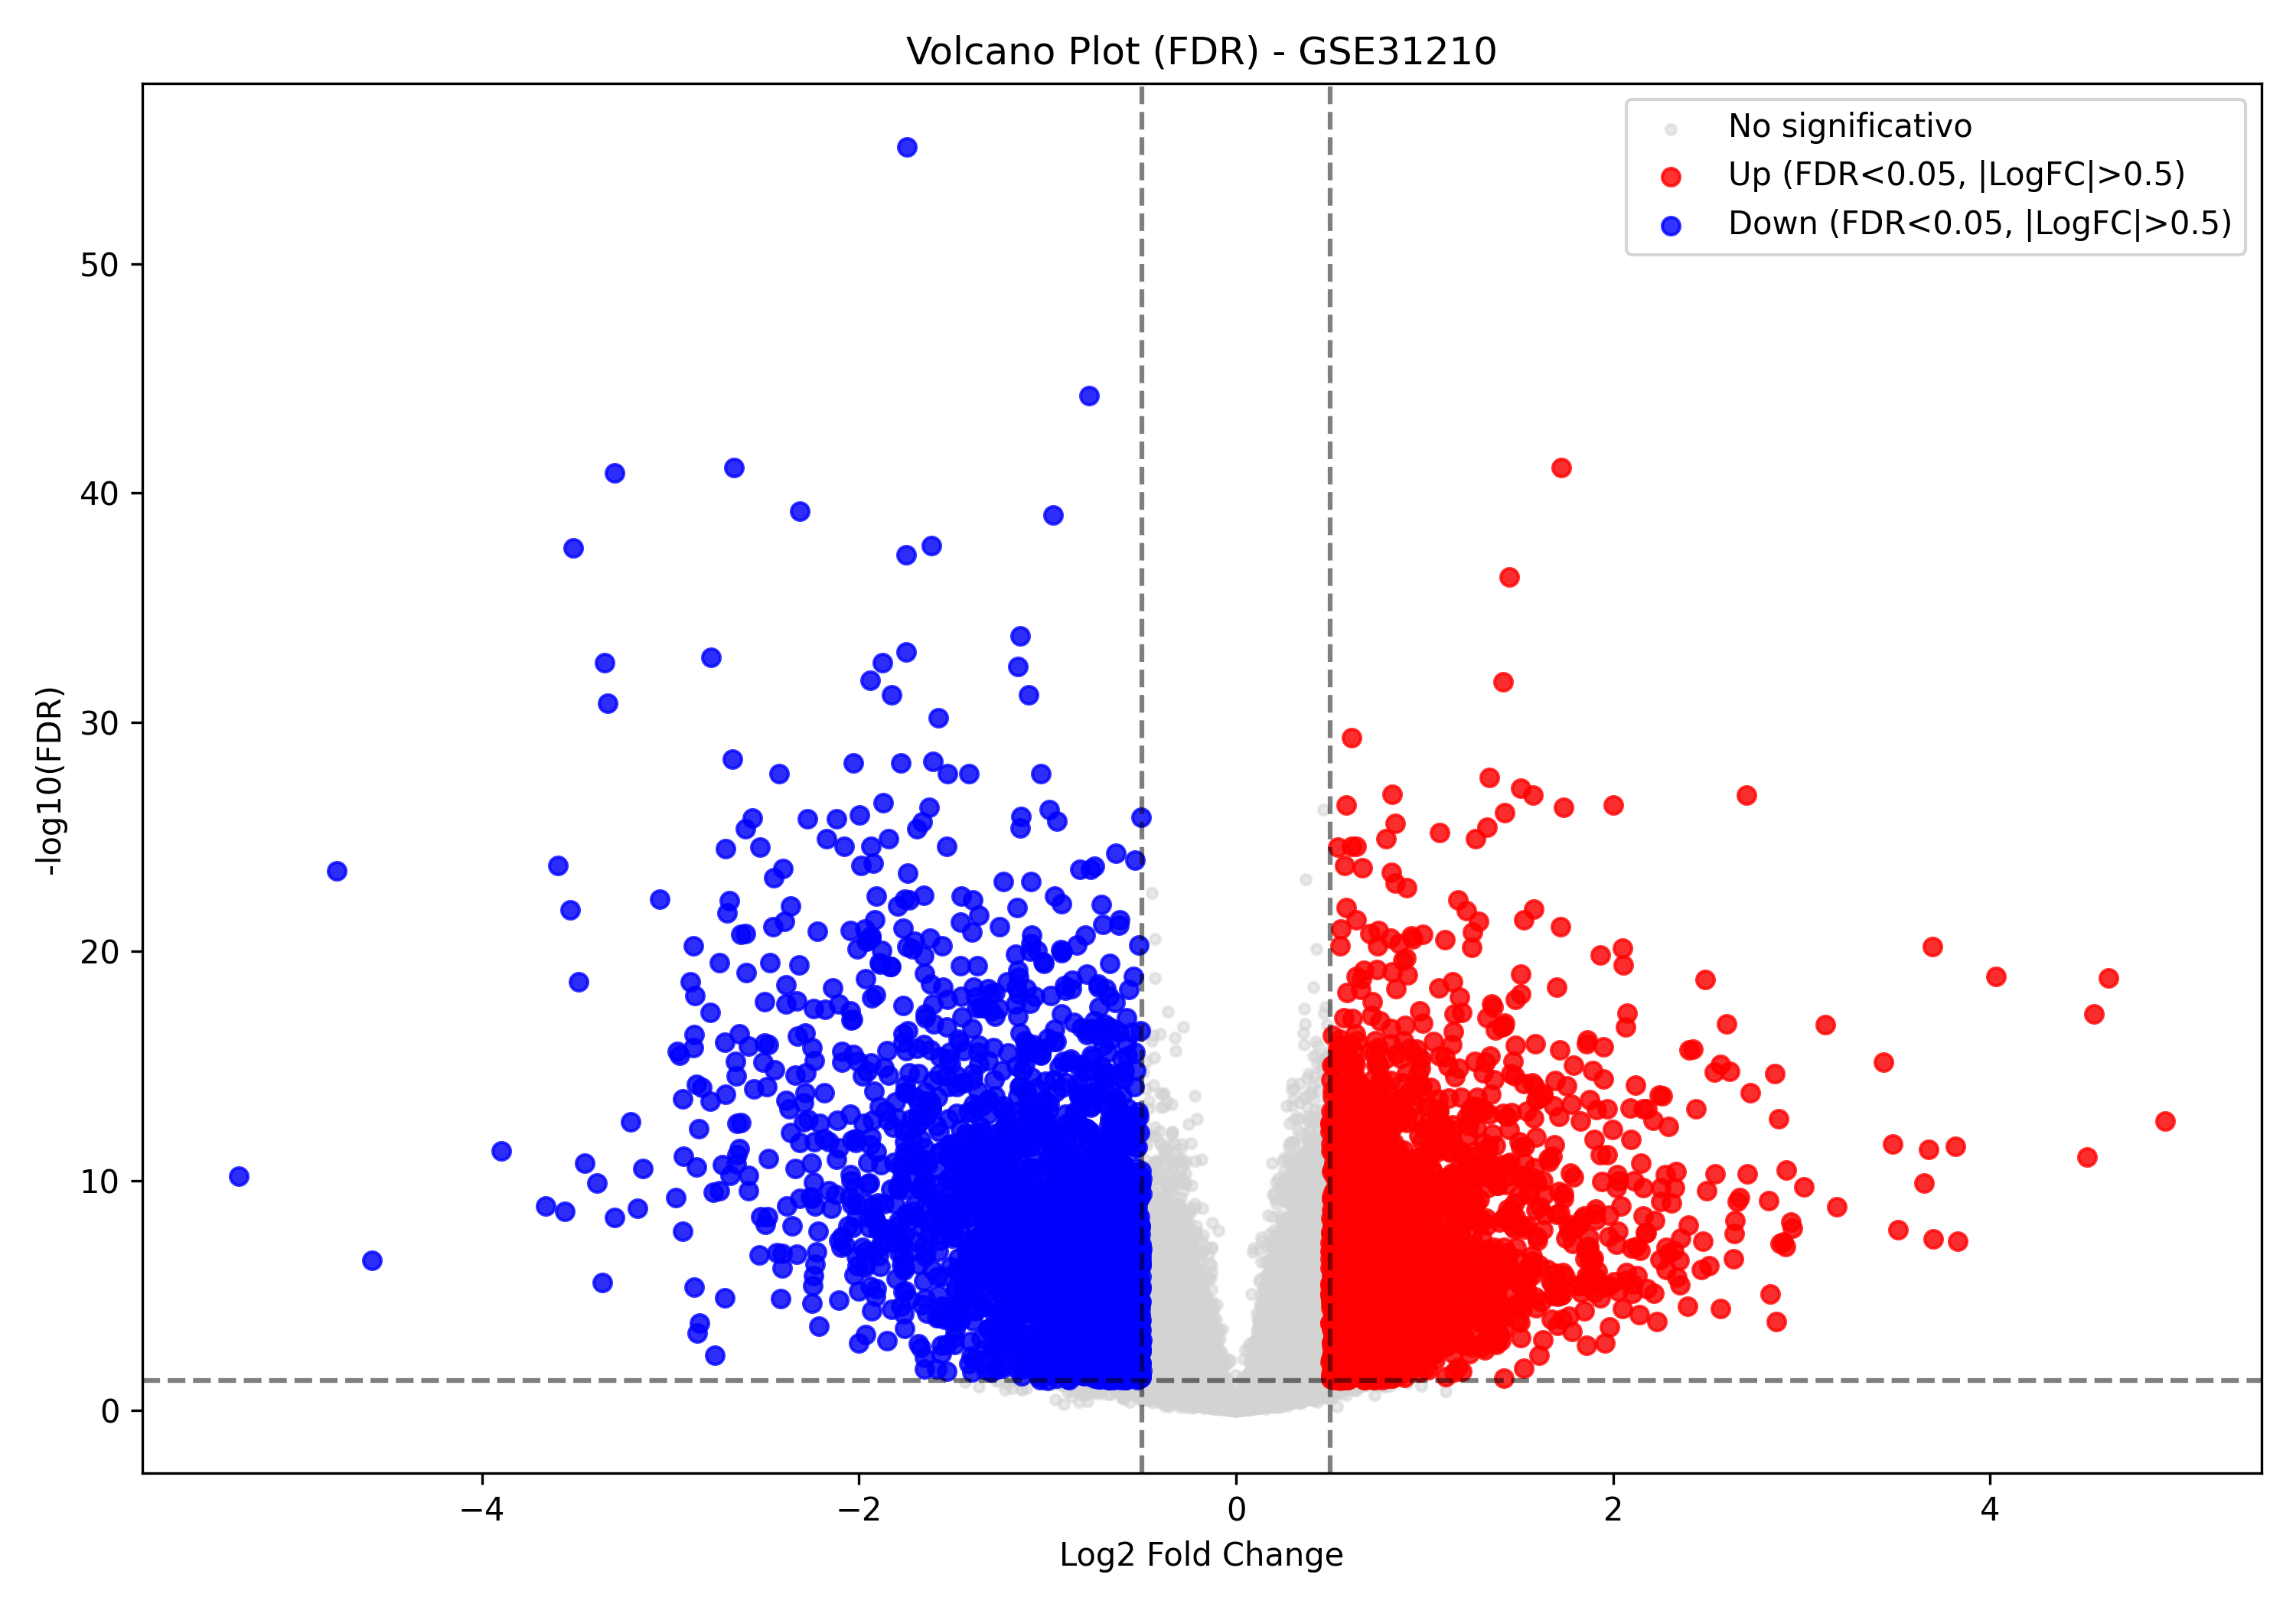
\includegraphics[width=\linewidth]{figuras/volcano_gse31210.png}
    \caption{Volcano plot}
  \end{subfigure}\hfill
  \begin{subfigure}[t]{0.31\textwidth}
    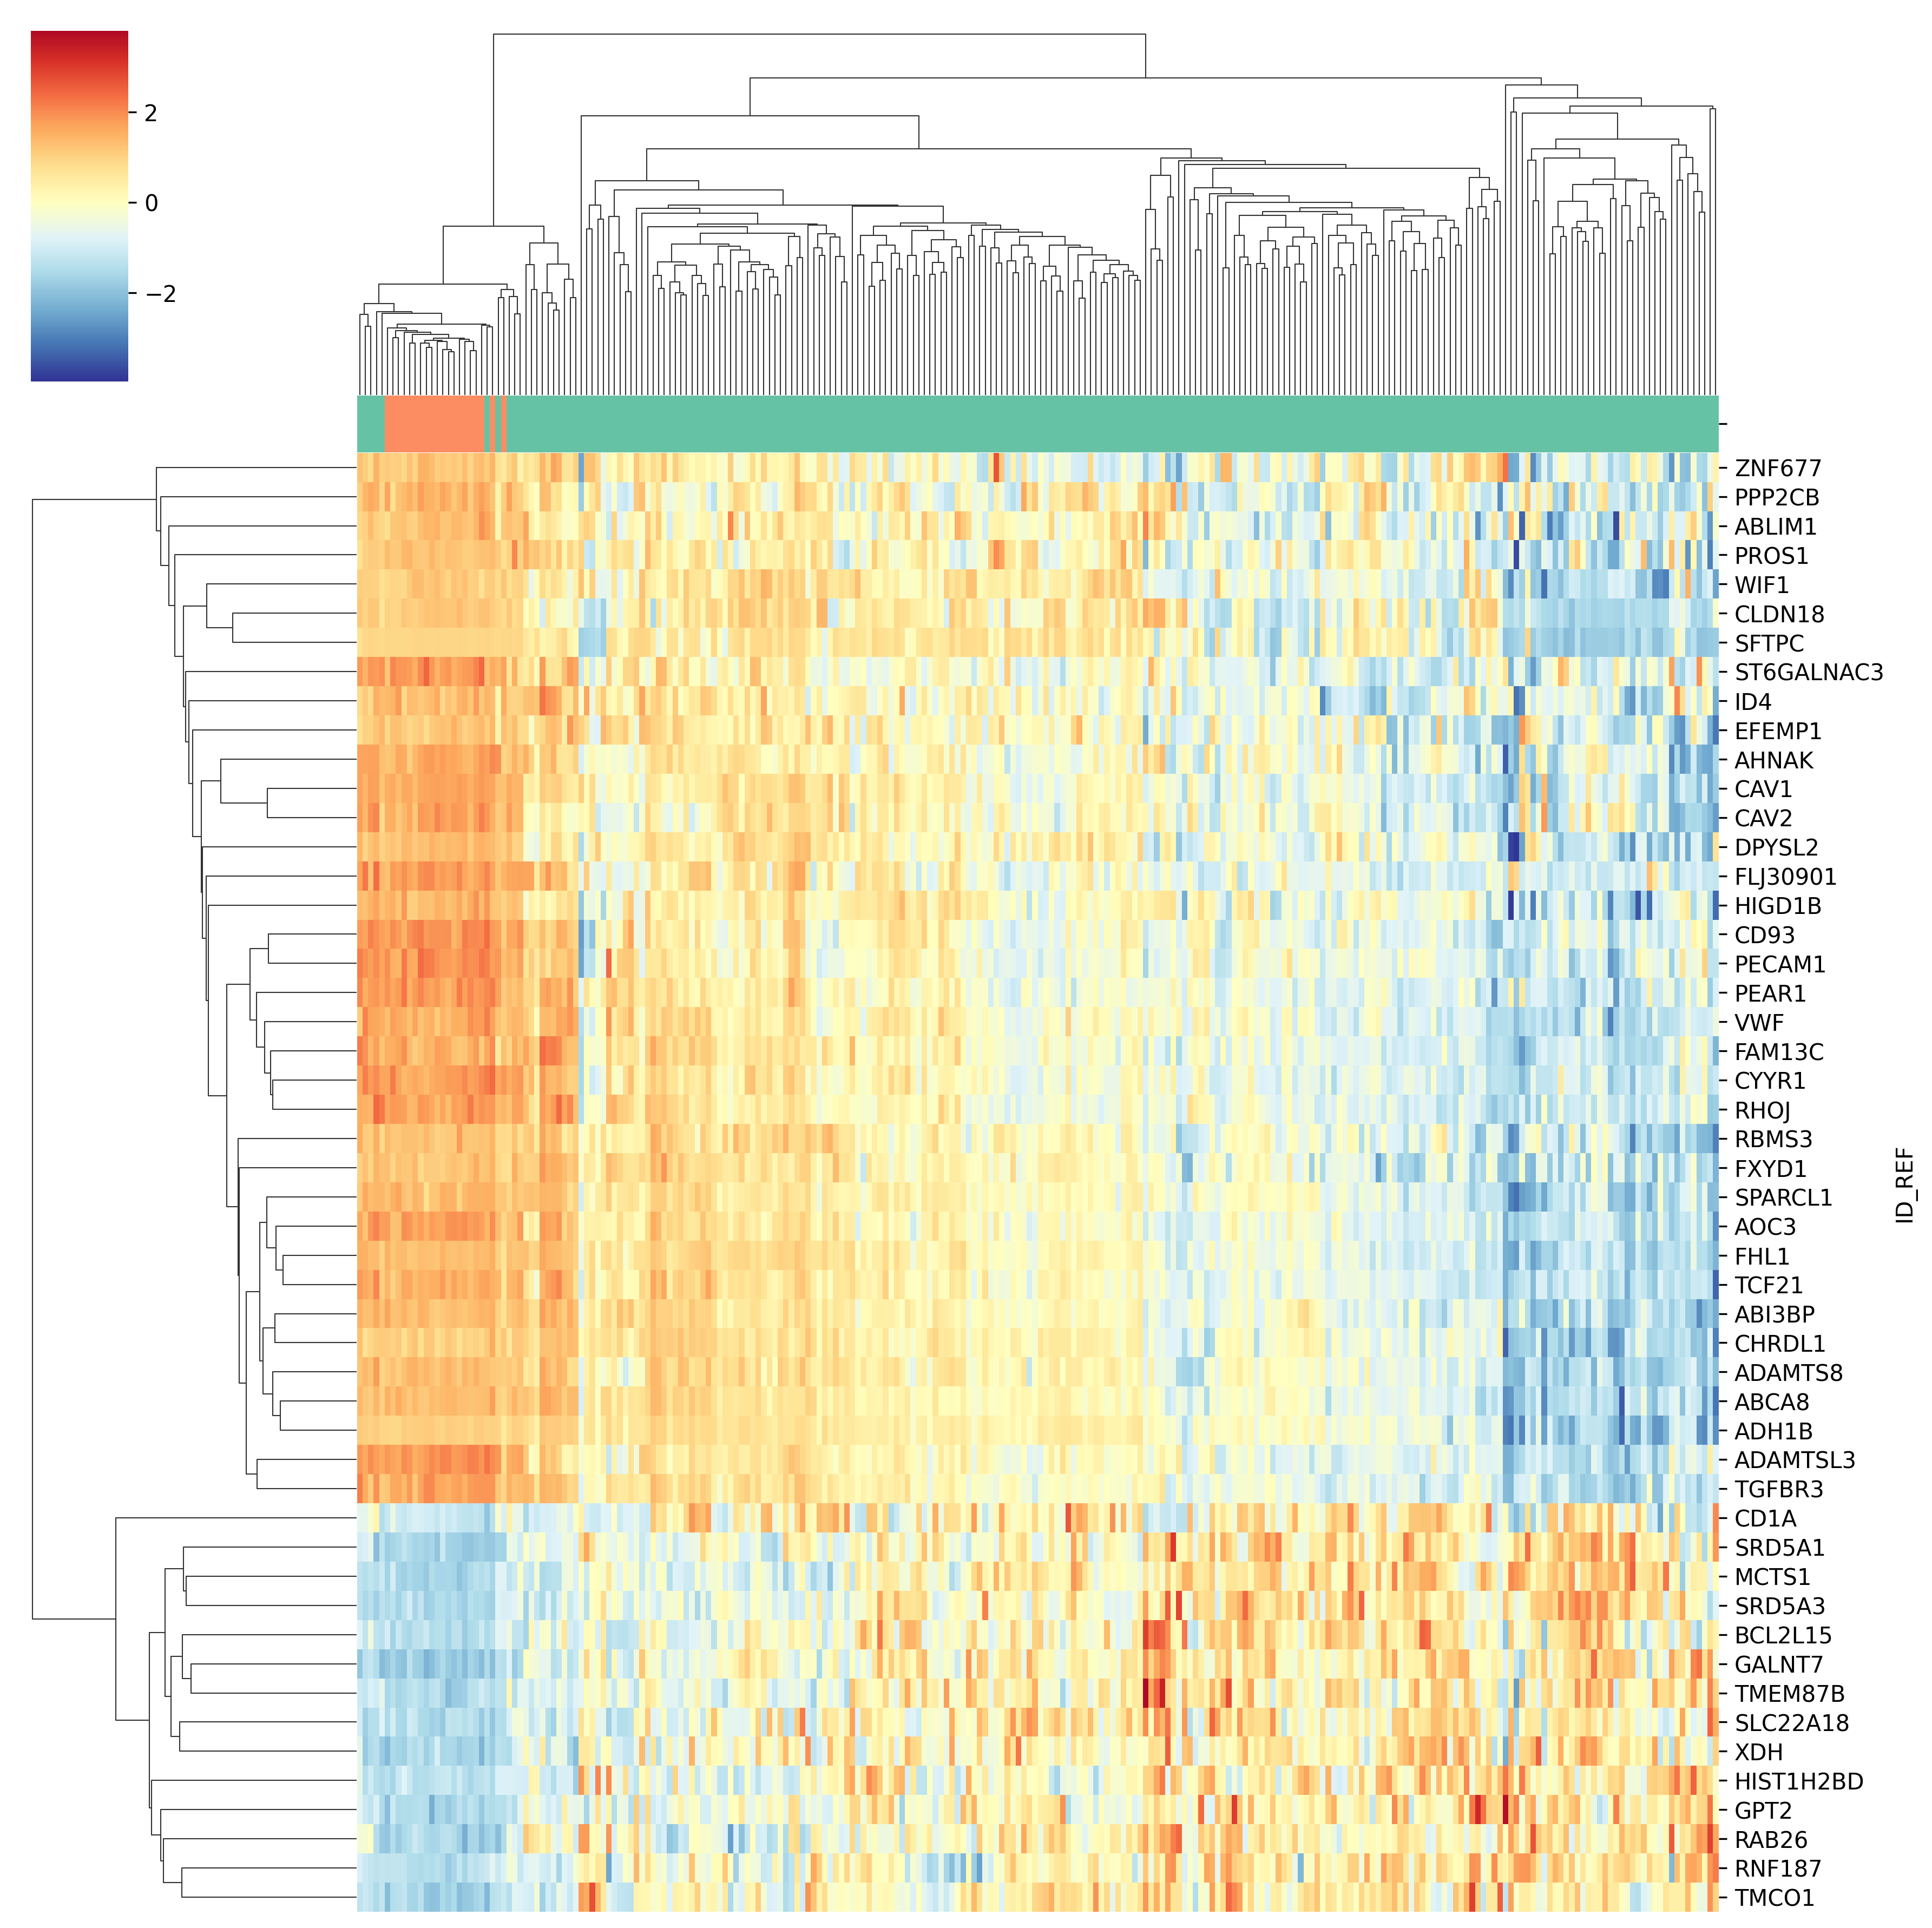
\includegraphics[width=\linewidth]{figuras/heatmap_gse31210.png}
    \caption{Heatmap}
  \end{subfigure}
  \caption{Análisis exploratorio de la cohorte GSE31210. (a) Componentes
  principales; los grupos sano y enfermo se separan en el plano.
  (b) Volcano de la comparación diferencial; miles de genes cruzan
  el umbral $|d|>1$ con FDR $<0{,}05$. (c) Heatmap de los 30 genes más
  significativos, con dendrograma de muestras que reproduce el grupo
  clínico.}
  \label{fig:cohorte}
\end{figure}

\section{Coherencia de los folds LODO}
\label{sec:res_coherencia}

Un último control comprueba que los genes seleccionados por LASSO en cada
fold LODO son consistentes entre iteraciones. La
figura~\ref{fig:concordancia} representa la concordancia de signos entre
folds. Un alto porcentaje de acuerdo en signo indica que la firma es
estable y no depende de qué cohorte concreta se retira como test.

\begin{figure}[H]
  \centering
  
\includegraphics[width=0.75\linewidth]{figuras/fig_concordancia_folds.pdf}
  \caption{Concordancia de signo de los coeficientes de LASSO entre
  distintos folds LODO. El acuerdo perfecto en signo se sitúa por encima
  del 90\,\% para los genes de la firma.}
  \label{fig:concordancia}
\end{figure}
